\documentclass{scrartcl}

\usepackage{amssymb}
\usepackage{amsmath}
\usepackage{wasysym} 
%\usepackage{musixtex}
%\usepackage{harmony}
\usepackage{tikz}
\usetikzlibrary{calc,intersections,through,backgrounds,patterns}
\usetikzlibrary{decorations.text, decorations.markings, fit, arrows, arrows.meta}
\usetikzlibrary{decorations.pathreplacing}	%for brackets

%from Barthes - S/Z, pp. 27-8, 29, 129

\begin{document}
	
	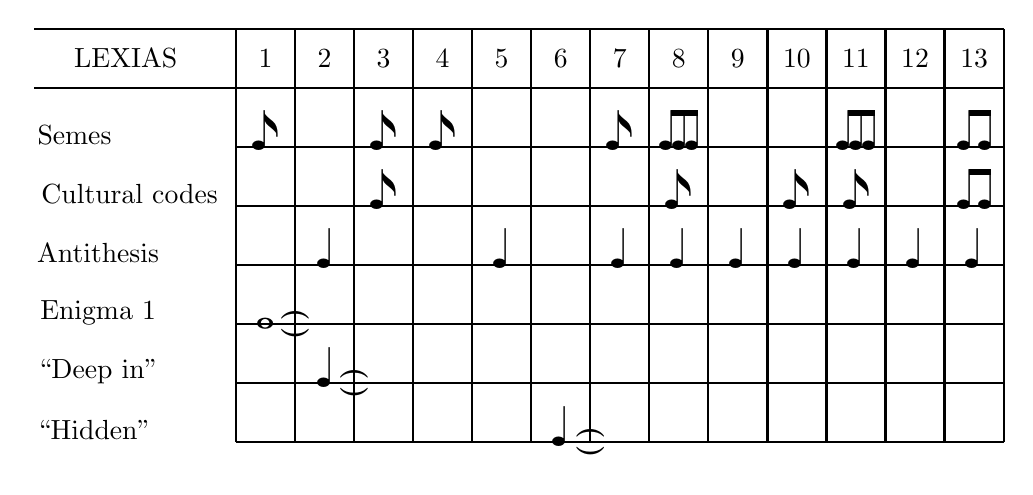
\begin{tikzpicture}
	\draw[step=0.75, thick] (0,0) grid (9.75,5.25);
		\draw[thick] (0,4.50)--(-2.57,4.50);
		\draw[thick] (0,5.25)--(-2.57,5.25);
	
	\node at (-1.4,4.875) {LEXIAS};
	\node at (-2.05,3.90) {Semes};
	\node at (-1.35,3.15) {Cultural codes};
	\node at (-1.75,2.40) {Antithesis};
	\node at (-1.75,1.65) {Enigma 1};
	\node at (-1.75,0.90) {``Deep in''};
	\node at (-1.8,0.15)  {``Hidden''};
	
	%for numbers, I should be able to write a `for' loop
	%for i in [1,13]
	%\node at ([0.375+0.75(i-1)],4.875) {[i]};
	
	\node at (0.375,4.875) {1};
	\node at (1.125,4.875) {2};
	\node at (1.875,4.875) {3};
	\node at (2.625,4.875) {4};
	\node at (3.375,4.875) {5};
	\node at (4.125,4.875) {6};
	\node at (4.875,4.875) {7};
	\node at (5.625,4.875) {8};
	\node at (6.375,4.875) {9};
	\node at (7.125,4.875) {10};
	\node at (7.875,4.875) {11};
	\node at (8.625,4.875) {12};
	\node at (9.375,4.875) {13};
	
	%full note
	\node at (0.375,1.5) {\huge \fullnote};
	
	%eighth notes
	\node at (0.375,3.95) {\huge \eighthnote};
	\node at (1.875,3.95) {\huge \eighthnote};
	\node at (2.625,3.95) {\huge \eighthnote};
	\node at (4.875,3.95) {\huge \eighthnote};
	%
	\node at (1.875,3.20) {\huge \eighthnote};
	\node at (5.625,3.20) {\huge \eighthnote};
	\node at (7.125,3.20) {\huge \eighthnote};
	\node at (7.875,3.20) {\huge \eighthnote};
	
	%quarter notes (wasysymb)
	\node at (1.12,2.45) {\huge \quarternote};
	\node at (3.35,2.45) {\huge \quarternote};
	\node at (4.85,2.45) {\huge \quarternote};
	\node at (5.60,2.45) {\huge \quarternote};
	\node at (6.35,2.45) {\huge \quarternote};
	\node at (7.10,2.45) {\huge \quarternote};
	\node at (7.85,2.45) {\huge \quarternote};
	\node at (8.60,2.45) {\huge \quarternote};
	\node at (9.35,2.45) {\huge \quarternote};
	%
	\node at (1.12,0.95) {\huge \quarternote};
	\node at (4.10,0.20) {\huge \quarternote};
	%\node at (3.375,2.25) {\musQuarter};			%musicography
	
	%three notes
	\node at (5.465,3.95) {\huge \quarternote};		%hack using wasysymb
	\node at (5.625,3.95) {\huge \quarternote};
	\node at (5.795,3.95) {\huge \quarternote};
		\draw[line width=2.1] (5.522,4.18)--(5.872,4.18);
	%
	\node at (7.715,3.95) {\huge \quarternote};
	\node at (7.875,3.95) {\huge \quarternote};
	\node at (8.045,3.95) {\huge \quarternote};
		\draw[line width=2.1] (7.772,4.18)--(8.122,4.18);
	
	%two notes
	%\node at (9.375,3.93) {\huge\twonotes};
	%\node at (9.375,3.18) {\huge\twonotes};
	%
	\node at (9.250,3.95) {\huge \quarternote};
	\node at (9.515,3.95) {\huge \quarternote};
		\draw[line width=2.1] (9.3068,4.18)--(9.5922,4.18);
	%
	\node at (9.250,3.20) {\huge \quarternote};
	\node at (9.515,3.20) {\huge \quarternote};
		\draw[line width=2.1] (9.3068,3.43)--(9.5922,3.43);
	%
	%\node at (9.375,3.87) {\AAcht};	%harmony package (straight, but too small)
	%\node at (9.375,3.12) {\AAcht};	%harmony package
	
	%brackets
	\node at (0.75,1.38) {\rotatebox{270}{\textbf{)}}};	%next to full note
	\node at (0.75,1.62) {\rotatebox{270}{\textbf{(}}};
	%
	\node at (1.5,0.63) {\rotatebox{270}{\textbf{)}}};	%next to col 2 quarter note
	\node at (1.5,0.87) {\rotatebox{270}{\textbf{(}}};
	%
	\node at (4.5,-0.12) {\rotatebox{270}{\textbf{)}}};	%next to col 6 quarter note
	\node at (4.5, 0.12) {\rotatebox{270}{\textbf{(}}};
	
	%lilyglyphs symbols
	%music note with tail: \quaver
	%plain note: \crotchet
	%three notes: \threeBeamedQuavers
	%two notes: \twoBeamedQuavers
	%circle: \wholeNote
	%brackets: \lilyGlyph{ties.lyric.short}
	
	%musicography symbols
	%music note with tail: \musEighth
	%plain note: \musQuarter
	%circle: \musWhole
	
	%harmony symbols -- NB: can't increase font size
	%note with tail: \Acht
	%plain note: \Vier
	%two notes: \AAcht
	
	\end{tikzpicture}
	
	
	
	\vspace{1.5cm}
	
	
	
	\hspace{1cm}
	%
	%
	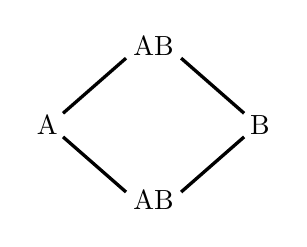
\begin{tikzpicture}
	\node at (-1.35,0) {A};
	\node at (1.35,0)  {B};
	\node at (0,1)     {AB};	%top
	\node at (0,-0.95) {AB};	%bottom
	
	\draw[very thick] (0.35,0.85)--(1.15,0.15);		%AB--B (top)
	\draw[very thick] (-0.35,0.85)--(-1.15,0.15);	%AB--A (top)
	\draw[very thick] (0.35,-0.85)--(1.15,-0.15);	%AB--B (bottom)
	\draw[very thick] (-0.35,-0.85)--(-1.15,-0.15);	%AB--A (bottom)
	\end{tikzpicture}
	%
	%
	\hspace{2cm}
	%
	%
	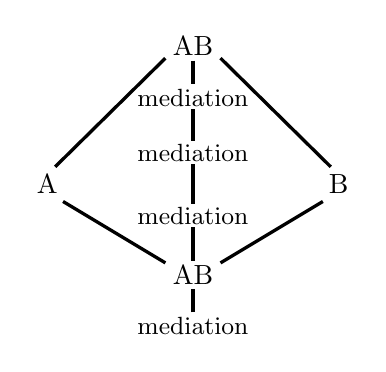
\begin{tikzpicture}
	\node at (-1.85,0) 	{A};
	\node at (1.85,0) 	{B};
	\node at (0,1.75) 	{AB};	%top
	\node at (0,-1.15) 	{AB};	%bottom
	
	\node at (0, 1.1) {{\small mediation}};
	\node at (0, 0.4) {{\small mediation}};
	\node at (0,-0.4) {{\small mediation}};
	\node at (0,-1.8) {{\small mediation}};
	
	%diagonal lines
	\draw[very thick]  (0.35,1.6)--(1.75,0.22);	 %AB--B (top)
	\draw[very thick] (-0.35,1.6)--(-1.75,0.22); %AB--A (top)
	\draw[very thick]  (0.35,-1)--(1.65,-0.22);	 %AB--B (bottom)
	\draw[very thick] (-0.35,-1)--(-1.65,-0.22); %AB--A (bottom)
	
	%vertical lines
	\draw[very thick] (0,1.57)--(0,1.27);
	\draw[very thick] (0,0.95)--(0,0.55);
	\draw[very thick] (0,0.25)--(0,-0.25);
	\draw[very thick] (0,-0.97)--(0,-0.55);
	\draw[very thick] (0,-1.63)--(0,-1.33);
	\end{tikzpicture}
	
	
	
	\vspace{1.5cm}
	
	
	
	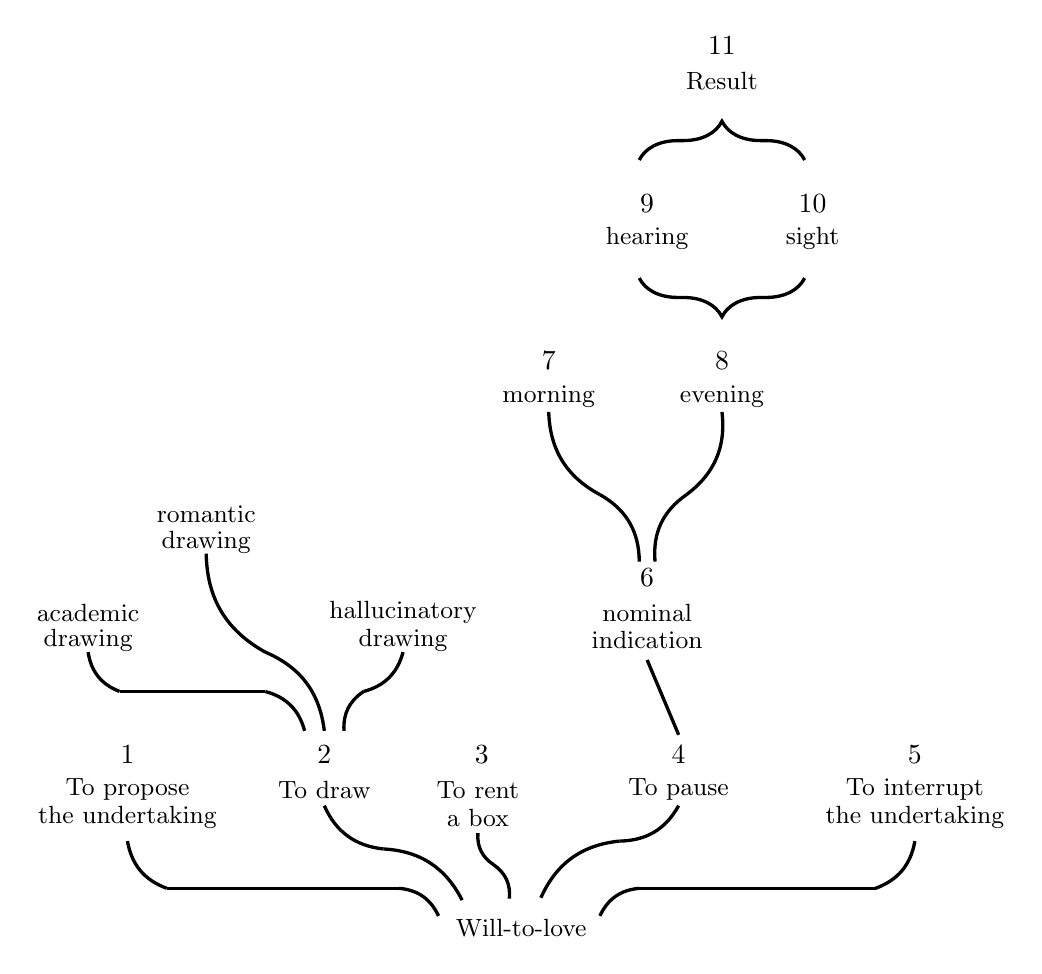
\begin{tikzpicture}
	\node at (0,0) {{\small Will-to-love}};
	%
	\node at (-5,1.75)    {{\small To propose}};
	\node at (-5,1.4)     {{\small the undertaking}};
	\node at (-2.5,1.75)  {{\small To draw}};
	\node at (-0.55,1.75) {{\small To rent}};
	\node at (-0.55,1.4)  {{\small a box}};
	\node at (2,1.75)     {{\small To pause}};
	\node at (5,1.75)     {{\small To interrupt}};
	\node at (5,1.4)      {{\small the undertaking}};
	%
	\node at (-5.5,4) 	 {{\small academic}};
	\node at (-5.5,3.65) {{\small drawing}};
	   \node at (-4,5.25){{\small romantic}};
	   \node at (-4,4.90){{\small drawing}};
	\node at (-1.5,4) 	 {{\small hallucinatory}};
	\node at (-1.5,3.65) {{\small drawing}};
	\node at (1.6,4) 	 {{\small nominal}};
	\node at (1.6,3.65)  {{\small indication}};
	%
	\node at (0.35,6.75) {{\small morning}};
	\node at (2.55,6.75) {{\small evening}};
	%
	\node at (1.6,8.75) {{\small hearing}};
	\node at (3.7,8.75) {{\small sight}};
	%
	\node at (2.55,10.75) {{\small Result}};
	
	\node at (-5,2.2) 	{1};
	\node at (-2.5,2.2) {2};
	\node at (-0.5,2.2) {3};
	\node at (2,2.2) 	{4};
	\node at (5,2.2) 	{5};
	\node at (1.6,4.45) {6};
	\node at (0.35,7.2) {7};
	\node at (2.55,7.2) {8};
	\node at (1.6,9.2)  {9};
	\node at (3.7,9.2)  {10};
	\node at (2.55,11.2){11};
	
	%bottom lines
	%\draw[very thick] (0,0)--(0,0);
	
	%\draw[very thick] (5,0) .. controls (6,0) and (6,1) .. (5,2);
	
	\draw[very thick] (-1.55,0.5)--(-4.5,0.5);					%Will--1
		\draw[very thick] (-1.05,0.15) to[bend right] (-1.55,0.5);
		\draw[very thick] (-4.5,0.5) to[bend left] (-5,1.1);
	
	\draw[very thick] (-0.75,0.35) to[bend right] (-1.75,1);	%Will--2
	\draw[very thick] (-1.75,1) to[bend left] (-2.5,1.55);
	
	\draw[very thick] (-0.15,0.37) to[bend right] (-0.35,0.8);	%Will--3
	\draw[very thick] (-0.35,0.8) to[bend left] (-0.55,1.2);
	
	\draw[very thick] (0.25,0.38) to[bend left] (1.25,1.1);		%Will--4
	\draw[very thick] (1.25,1.1) to[bend right] (2,1.55);
	
	\draw[very thick] (1.5,0.5)--(4.5,0.5);						%Will--5
		\draw[very thick] (1,0.15) to[bend left] (1.5,0.5);
		\draw[very thick] (4.5,0.5) to[bend right] (5,1.1);
	
	%middle lines
	\draw[very thick] (-3.25,3)--(-5.1,3);						%2--academic
		\draw[very thick] (-5.1,3) to[bend left] (-5.5,3.5);
		\draw[very thick] (-3.25,3) to[bend left] (-2.75,2.5);
	
	\draw[very thick] (-2.5,2.5) to[bend right] (-3.25,3.5);	%2--romantic
	\draw[very thick] (-3.25,3.5) to[bend left] (-4,4.75);
	
	\draw[very thick] (-2.25,2.5) to[bend left] (-2,3);			%2--hallucinatory
	\draw[very thick] (-2,3) to[bend right] (-1.5,3.5);
	
	\draw[very thick] (2,2.45)--(1.6,3.4);  					%4--6
	
	%upper lines	
	\draw[very thick] (1.5,4.65) to[bend right] (1,5.5);		%6--7
	\draw[very thick] (1,5.5) to[bend left] (0.35,6.55);
	
	\draw[very thick] (1.7,4.65) to[bend left] (2.1,5.5);		%6--8
	\draw[very thick] (2.1,5.5) to[bend right] (2.55,6.55);
	
	%top brackets
	\draw[decorate,decoration={brace,amplitude=14pt},yshift=0pt,very thick] (3.6,8.25)--(1.5,8.25);
	\draw[decorate,decoration={brace,amplitude=14pt},yshift=0pt,very thick] (1.5,9.75)--(3.6,9.75);
	
	%\node at (2.55,7.75) {\rotatebox{90}{$\left\{ \rule{0pt}{12mm}\right.$}};  %8--{9,10
	%\node at (2.65,10) {\rotatebox{270}{$\left\{ \rule{0pt}{12mm}\right.$}};  %{9,10--11
	
	%\draw[help lines] (-6,0) grid (6,11);
	\end{tikzpicture}
	
\end{document}